\section{Resultados y an\'alisis de resultados}

\subsection{Caracter\'isticas del conjunto de datos original}
El conjunto tabular contiene \cifNEstudios{} estudios en \texttt{train.csv}: \cifPos{} con fractura (\texttt{patient\_overall}\,=\,1; 47.6\,\%) y \cifNeg{} sin fractura. Solo 235 estudios (11.6\,\%) cuentan con \emph{bounding boxes} (7\,217 anotaciones), todas en estudios positivos (primera entrega del Proyecto~2). Las im\'agenes son estudios de TC en formato DICOM con entre \cifNCortesMin{} y \cifNCortesMax{} cortes por estudio (mediana \cifNCortesMed{}).

\begin{figure}[H]\centering
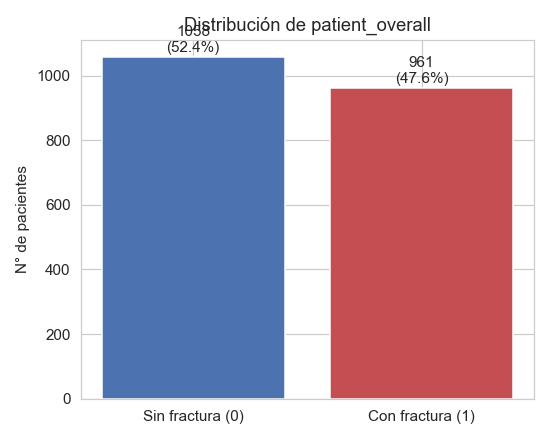
\includegraphics[width=.48\linewidth]{01_patient_overall.png}\hfill
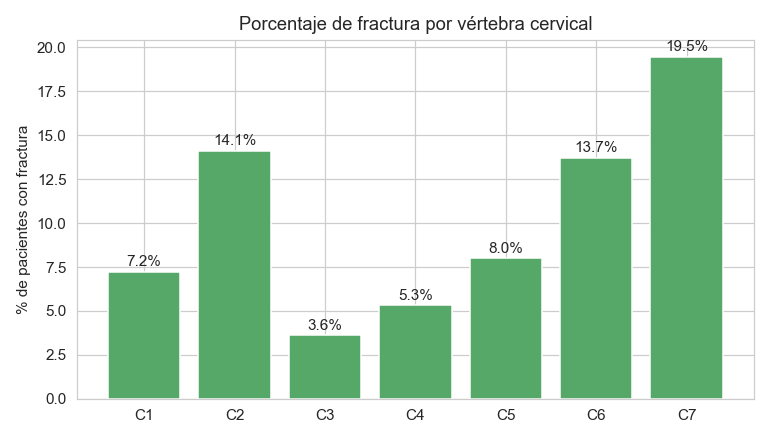
\includegraphics[width=.48\linewidth]{02_frac_por_vertebra.png}
\caption{An\'alisis exploratorio tabular (primera entrega): distribuci\'on de la variable objetivo \texttt{patient\_overall} y frecuencia de fractura por v\'ertebra.}
\end{figure}

\subsection{Limpieza y preprocesamiento}
En los CSV no hubo valores nulos ni filas duplicadas, \texttt{StudyInstanceUID} es \'unico y \texttt{patient\_overall} es consistente con la suma de C1--C7, por lo que no se aplicaron correcciones a las etiquetas. En las im\'agenes, la variabilidad de metadatos no se corrige en los archivos sino en el \emph{pipeline} (secci\'on~\ref{sec:eda-dicom}): HU calculadas con el \texttt{RescaleSlope}/\texttt{RescaleIntercept} de cada archivo, ordenamiento por posici\'on $z$ y redimensionado a $224\times224$.

\subsection{An\'alisis exploratorio de las im\'agenes DICOM}\label{sec:eda-dicom}
\paragraph{Fuente y tama\~no de muestra.} El an\'alisis usa la auditor\'ia del \emph{pipeline} (\cifFuente): \cifNEstudios{} estudios y \cifCortesLeidos{} cortes (los 48 centrales de cada estudio). El n\'umero de cortes por estudio es el total de archivos del estudio; el resto de metadatos proviene \'unicamente de esos 48 cortes. El notebook \texttt{notebooks/02\_eda\_imagenes.ipynb} y el script \texttt{scripts/eda\_metadatos\_dicom.py} permiten repetir el an\'alisis leyendo las cabeceras de \emph{todos} los cortes de una muestra estratificada (semilla 42) directamente en Kaggle.

\paragraph{Estad\'istica descriptiva.}
\begin{table}[H]\centering\small\tablaDesc
\caption{Estad\'istica descriptiva por estudio (\cifNEstudios{} estudios).}
\end{table}
El grosor de corte toma pocos valores discretos (mediana 0.625~mm, m\'aximo 1~mm, en l\'inea con el criterio de inclusi\'on del conjunto de datos de grosor $\le 1$~mm; \citealp{lin2023rsna}), mientras que el tama\~no de p\'ixel var\'ia entre 0.19 y 0.713~mm; el n\'umero de cortes cubre un rango de m\'as de un orden de magnitud. Tras redimensionar a $224\times224$, el tama\~no f\'isico del p\'ixel resultante var\'ia entre estudios, pues no se remuestrea de forma isotr\'opica.

\begin{figure}[H]\centering
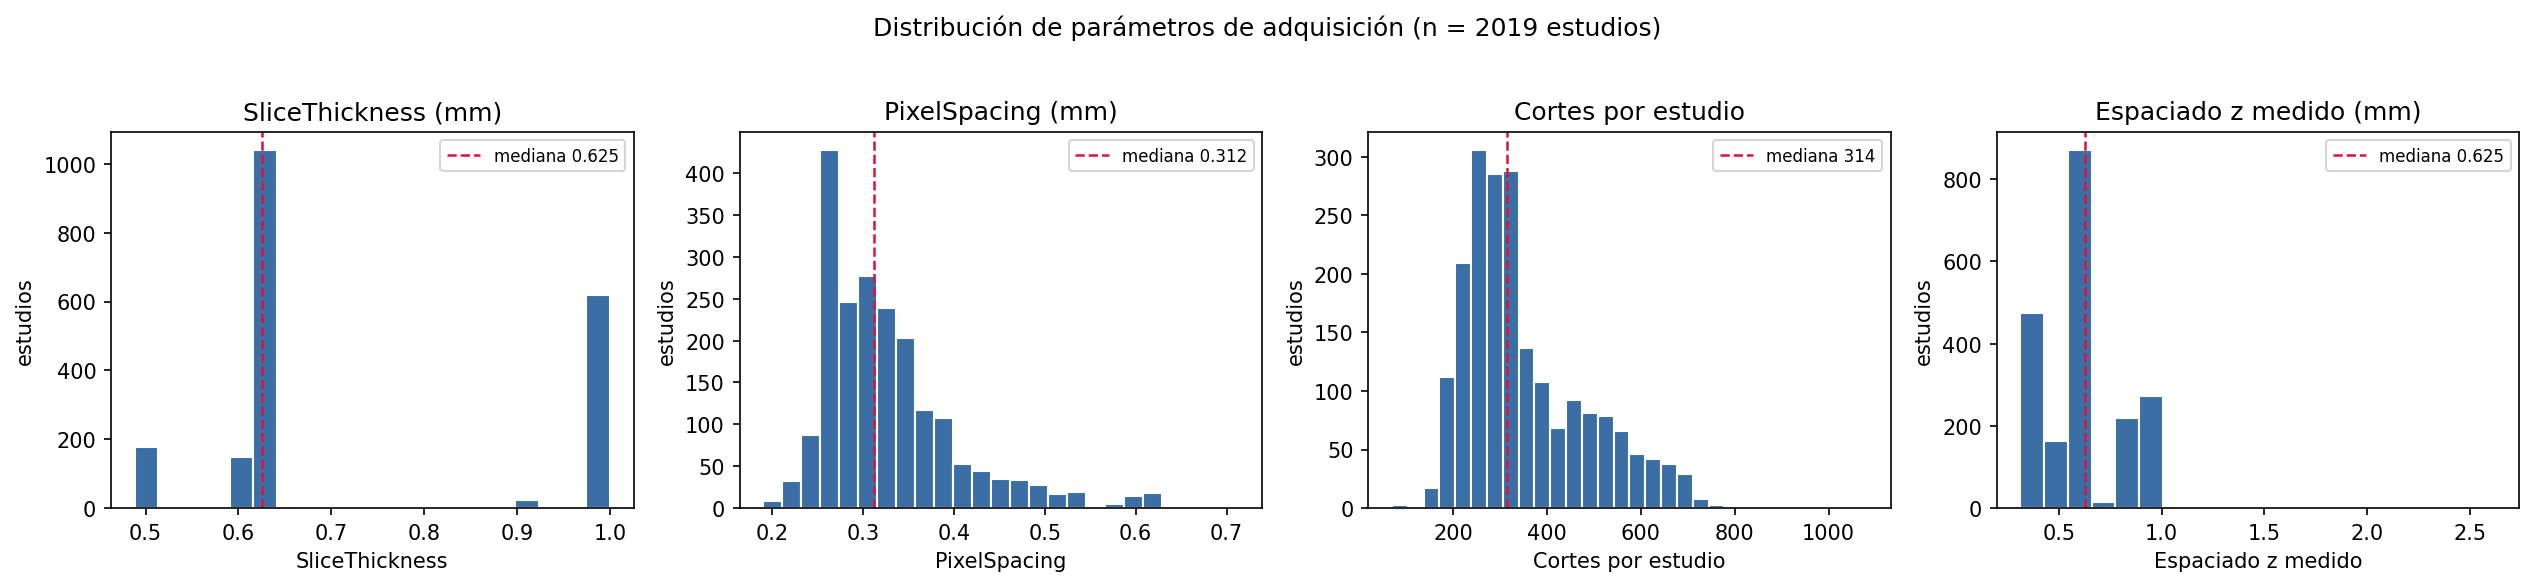
\includegraphics[width=\linewidth]{01_distribuciones_adquisicion.png}
\caption{Distribuciones de cortes por estudio, SliceThickness, PixelSpacing y espaciado $z$ medido.}
\end{figure}
\begin{figure}[H]\centering
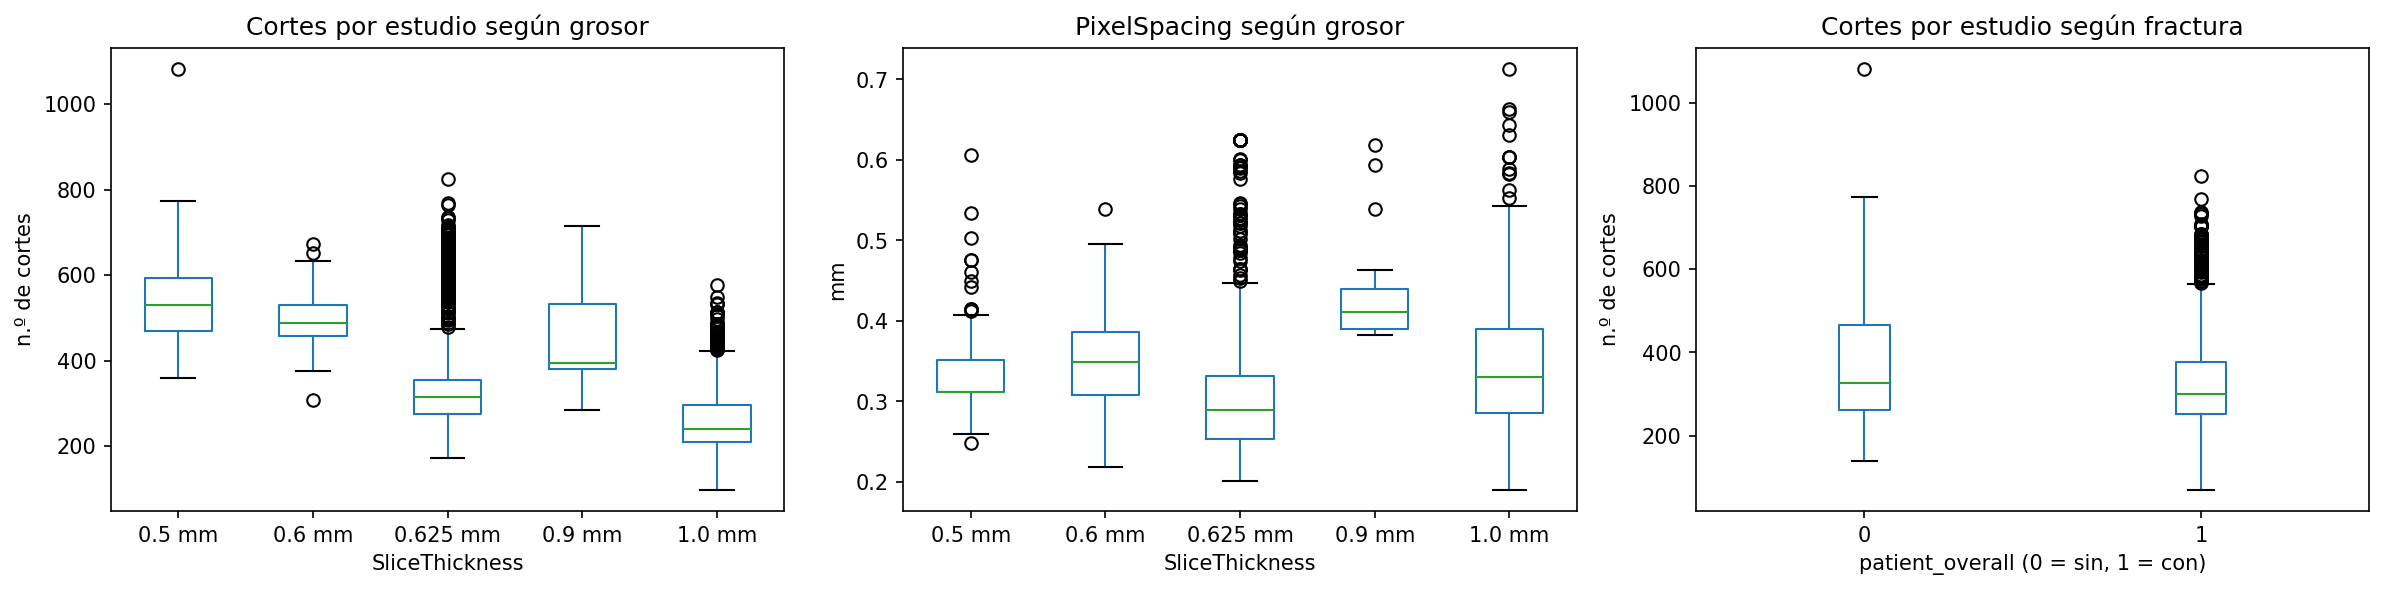
\includegraphics[width=\linewidth]{02_boxplots_comparacion.png}
\caption{Comparaci\'on de par\'ametros de adquisici\'on seg\'un \texttt{patient\_overall} (descriptiva; sin prueba de hip\'otesis).}
\end{figure}
\begin{figure}[H]\centering
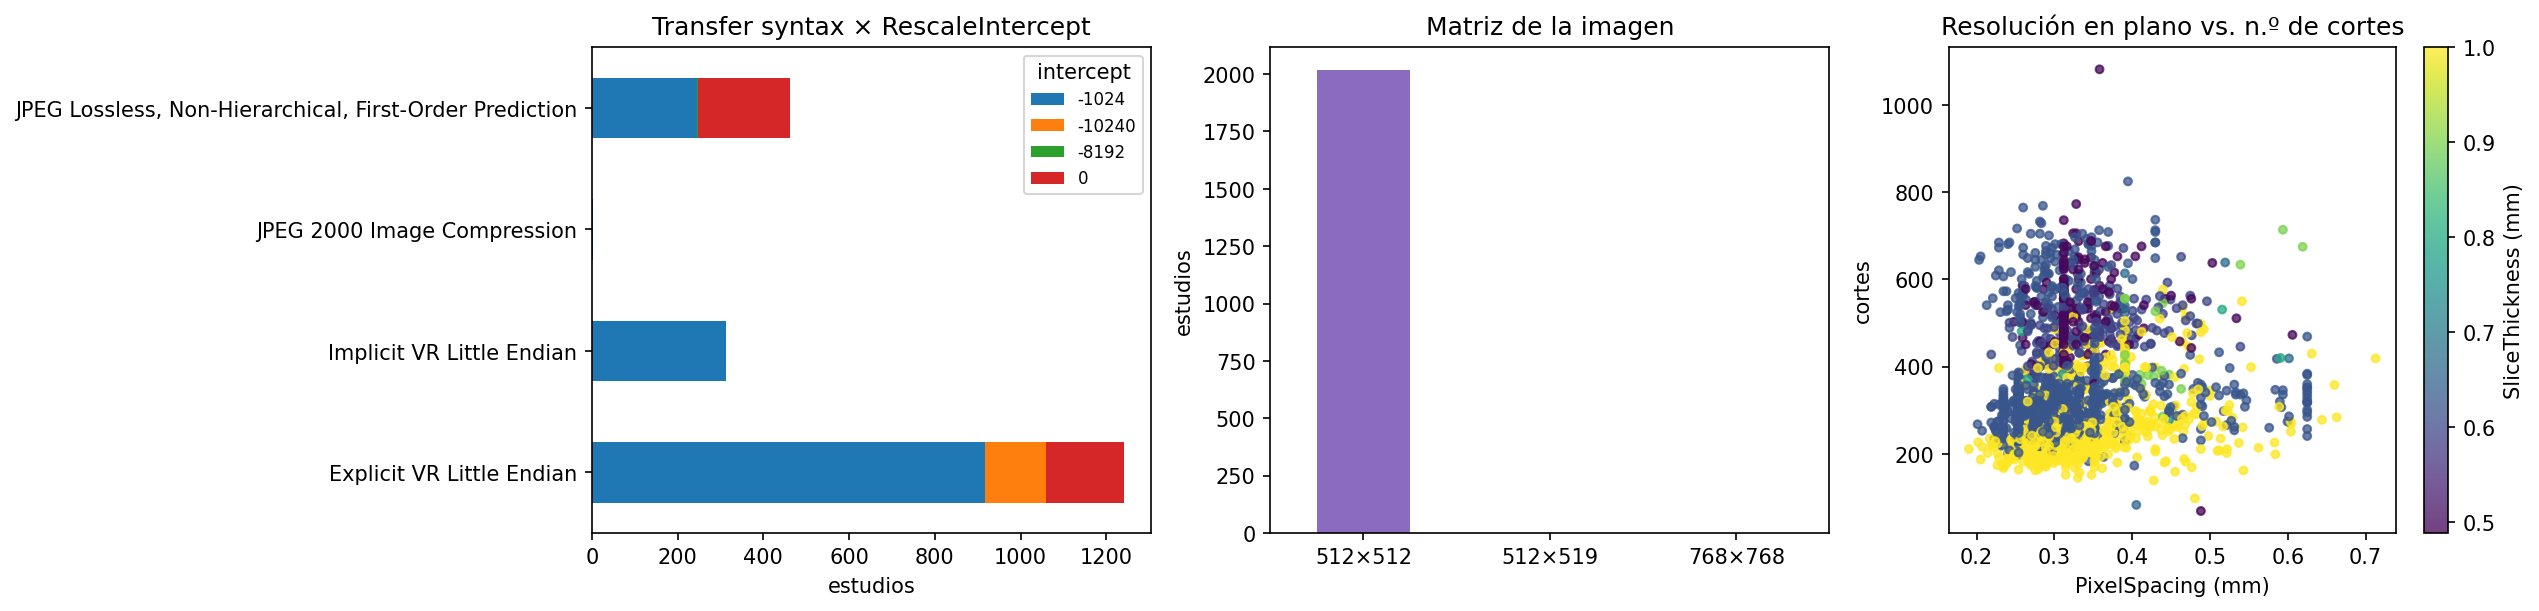
\includegraphics[width=\linewidth]{03_protocolos_y_resolucion.png}
\caption{Protocolos de reescalado, sintaxis de transferencia y resoluci\'on de matriz.}
\end{figure}

\paragraph{Valores at\'ipicos y metadatos inconsistentes.}
\begin{table}[H]\centering\small\tablaChecks
\caption{Comprobaciones de calidad sobre los metadatos. Los umbrales de at\'ipicos usan IQR$\times$1.5.}
\end{table}
Los hallazgos relevantes para el preprocesamiento son: (i) \cifNInterceptAtip{} estudios (\cifNInterceptAtipPct\,\%) con \texttt{RescaleIntercept} distinto de $-1024$ y $0$: 141 con intercept $-10240$ y \texttt{RescaleSlope} $=10$, y 3 con intercept $-8192$; (ii) \cifNNoQuinientos{} estudios que no son $512\times512$; (iii) ning\'un estudio con dimensiones, grosor o reescalado variables \emph{dentro} del estudio, ni fotometr\'ia distinta de MONOCHROME2; (iv) \cifNOutPixel{} estudios con \texttt{PixelSpacing} at\'ipico y \cifNOutCortes{} con n\'umero de cortes at\'ipico. Que las HU resultantes de los estudios con reescalado at\'ipico sean plausibles se comprueba con p\'ixeles reales y no con metadatos (v\'ease m\'as abajo).

\paragraph{Orden de los cortes y auditor\'ia del \emph{pipeline}.}
El sentido de $z$ respecto al n\'umero de instancia no es constante: \cifZDecr{} estudios son decrecientes, \cifZCrec{} crecientes y \cifZMixto{} mixto; \cifZNoMono{} estudio no es mon\'otono. Los estudios con espaciado $z$ irregular o no mon\'otono son \cifZAnomalos{} (identificados por los \'ultimos d\'igitos de su UID). Esto justifica ordenar por \texttt{ImagePositionPatient[2]} y no por n\'umero de instancia. El sentido creciente es m\'as frecuente en estudios positivos (\cifPosCrecPct\,\% frente a \cifNegCrecPct\,\% en negativos; $\chi^2$, $p=\cifChiP$); es una asociaci\'on descriptiva que podr\'ia reflejar diferencias de protocolo o instituci\'on, que los metadatos disponibles no permiten confirmar.
El preprocesamiento de los \cifNEstudios{} estudios termin\'o con \cifFallosPrep{} fallos; el tiempo por estudio fue de \cifTMedia{}~s en promedio (mediana \cifTMediana{}~s, m\'aximo \cifTMax{}~s) y los estudios comprimidos con JPEG Lossless tardaron aproximadamente el doble que los no comprimidos (mediana 4.07~s frente a 2.11~s con Explicit VR Little Endian).

\begin{figure}[H]\centering
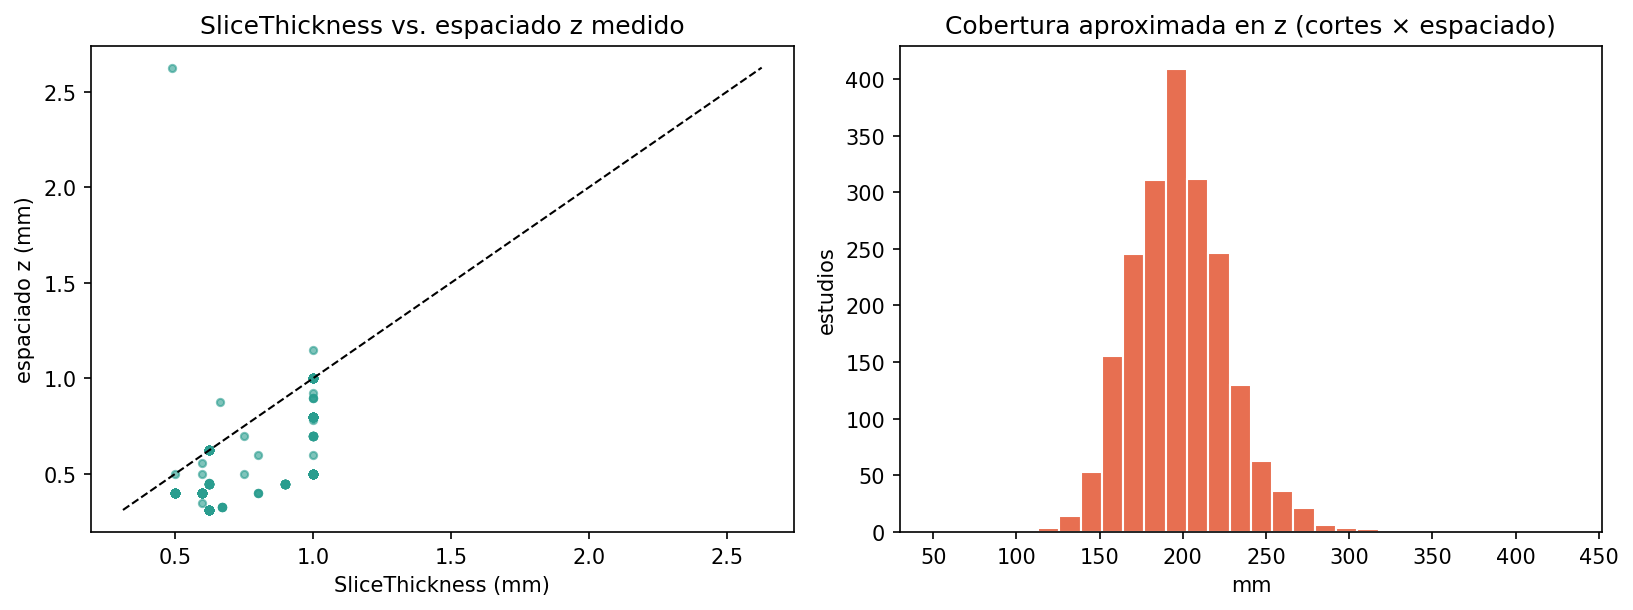
\includegraphics[width=\linewidth]{04_consistencia_z.png}
\caption{Consistencia del eje $z$ entre estudios.}
\end{figure}
\begin{figure}[H]\centering
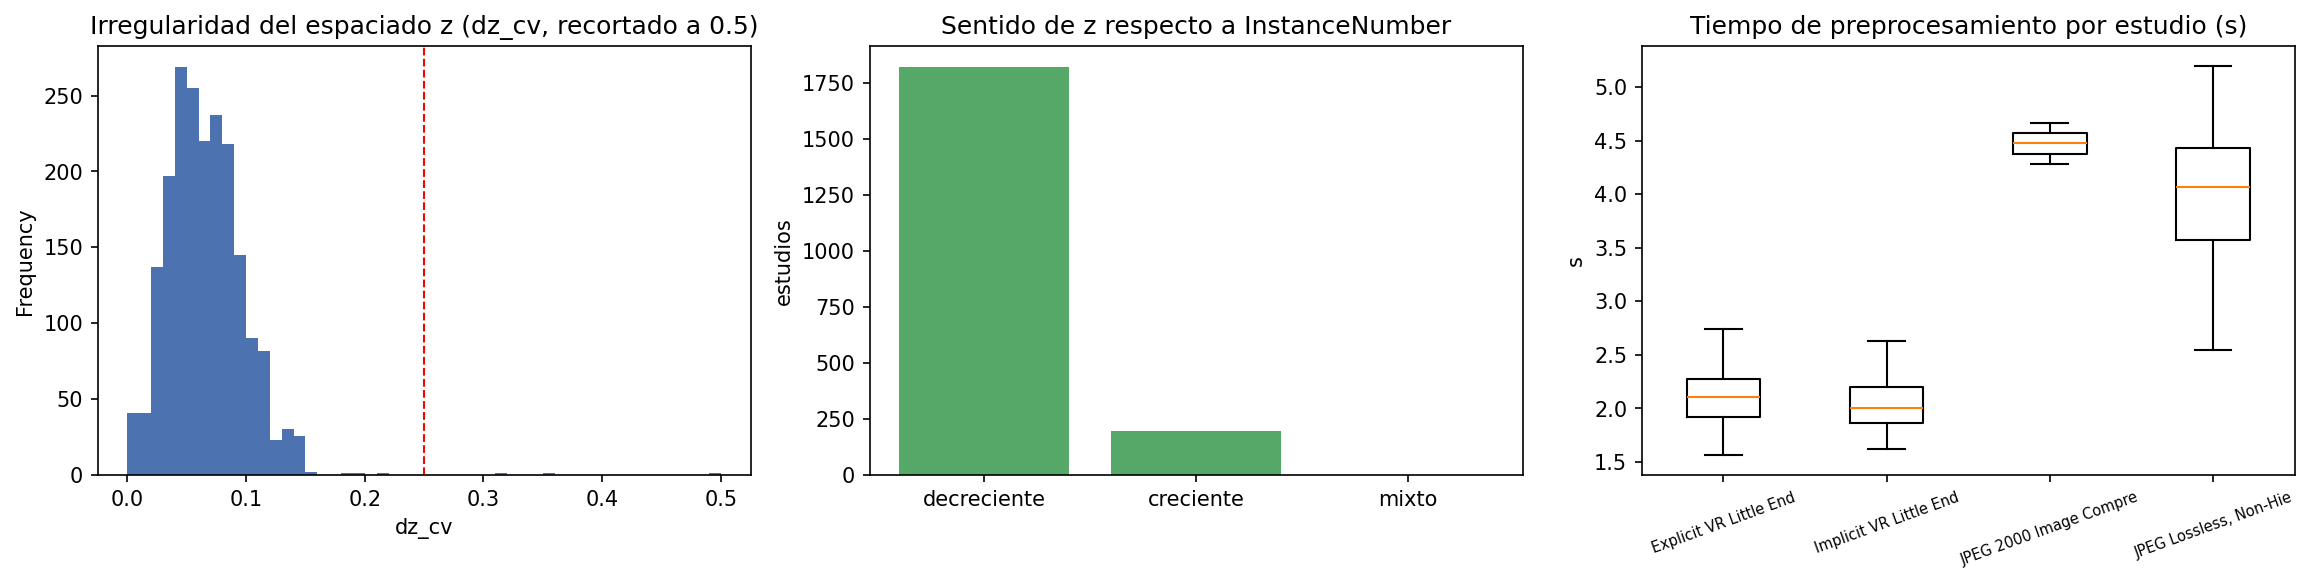
\includegraphics[width=\linewidth]{07_auditoria_pipeline.png}
\caption{Auditor\'ia del \emph{pipeline}: irregularidad del espaciado $z$, sentido de $z$ y tiempo de preprocesamiento por sintaxis de transferencia.}
\end{figure}

\paragraph{Ejemplos reales antes y despu\'es del preprocesamiento.}
Las figuras siguientes provienen del \emph{pipeline} de entrenamiento (\texttt{artifacts/v2/results/figures/}) y muestran el corte en HU crudo, el histograma con la ventana \'osea y el resultado final.
\begin{figure}[H]\centering
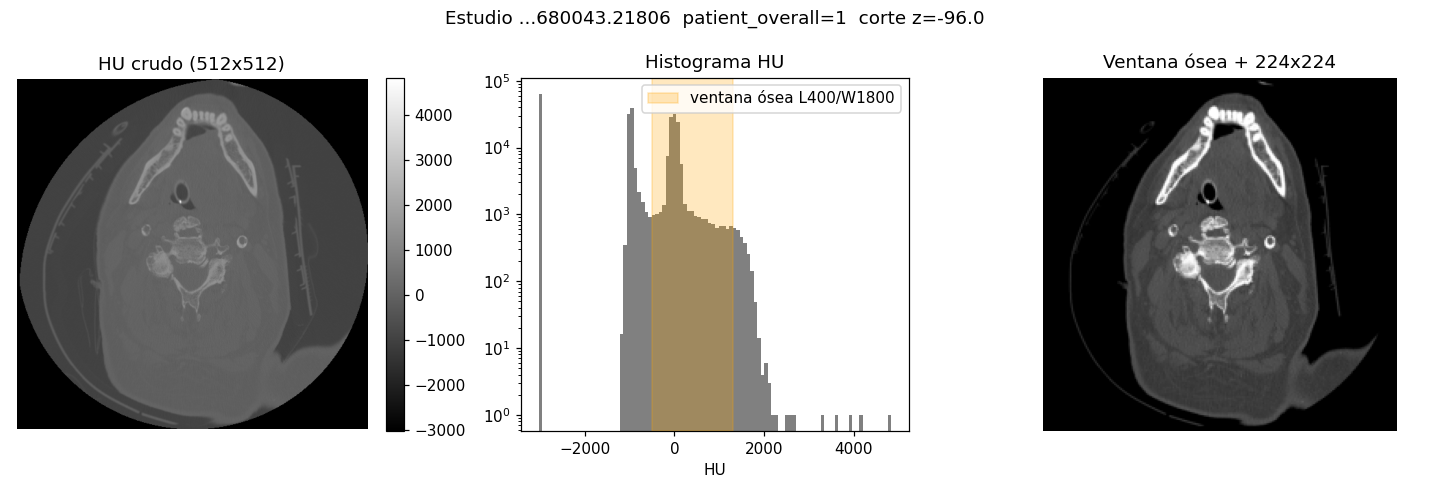
\includegraphics[width=\linewidth]{preproc_antes_despues_y1_21806.png}\\[3pt]
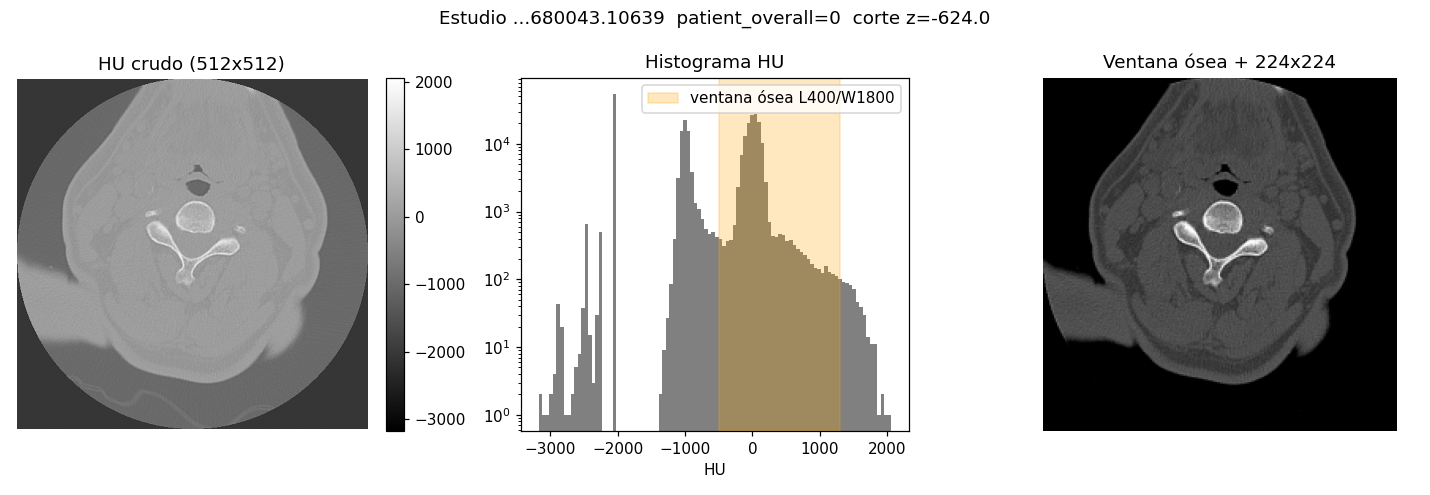
\includegraphics[width=\linewidth]{preproc_antes_despues_y0_10639.png}
\caption{Antes y despu\'es del preprocesamiento en un estudio positivo (arriba) y uno negativo (abajo).}
\end{figure}
\pendiente{Intensidades (HU) por grupo de reescalado y diferencias de adquisici\'on}{Histogramas de HU del corte central de una submuestra, con todos los estudios de reescalado at\'ipico y estudios aleatorios, y la comparaci\'on antes/despu\'es sobre ellos (secci\'on~5 del notebook 02).}{Ejecuci\'on de \texttt{notebooks/02\_eda\_imagenes.ipynb} en Kaggle con la competencia como entrada (produce \texttt{intensidades\_corte\_central.csv} y las figuras 05 y 06).}

\paragraph{Limitaciones del EDA de im\'agenes.}
\begin{itemize}[nosep]
\item Solo se dispone de las cabeceras de 48 cortes centrales por estudio; no se pueden detectar huecos en $z$ ni cabeceras at\'ipicas fuera de esos cortes.
\item El espaciado $z$ medido es la distancia entre dos cortes consecutivos \emph{muestreados}, no una mediana del estudio. Por ello la comparaci\'on grosor\,\,vs.\,\,espaciado $z$ (\cifNGrosorSpacing{} estudios, \cifNGrosorSpacingPct\,\%) no es concluyente y se excluye de la tabla de calidad hasta confirmarla con cabeceras completas.
\item Las comprobaciones sobre cabeceras no sustituyen una revisi\'on cl\'inica de la calidad de imagen ni miden artefactos (metal, movimiento).
\item La comparaci\'on por \texttt{patient\_overall} es descriptiva, sin control de confusores de protocolo.
\end{itemize}

\subsection{Ajuste de par\'ametros}
\pendiente{Ajuste de par\'ametros de cada algoritmo (responsable GPU)}{Qu\'e par\'ametros se ajustaron, c\'omo y con qu\'e efecto sobre el rendimiento.}{Texto de la responsable GPU; historiales en \texttt{artifacts/v2/results/history\_*.csv}.}

\subsection{Comparaci\'on de algoritmos}
\pendiente{Comparaci\'on de modelos y selecci\'on (P3)}{Tabla comparativa de m\'etricas, pruebas estad\'isticas pareadas, tiempos y figuras est\'aticas (ROC, matrices de confusi\'on, distribuci\'on de probabilidades) con interpretaci\'on y modelo seleccionado.}{An\'alisis y redacci\'on de P3 (Hansel); datos en \texttt{artifacts/v2/results/} y \texttt{notebooks/03\_evaluacion.ipynb} (rama \texttt{main}).}

\subsection{Aplicaci\'on desarrollada}
\pendiente{Aplicaci\'on Streamlit (P1)}{Descripci\'on de la aplicaci\'on, capturas de pantalla y justificaci\'on de las tecnolog\'ias elegidas.}{Capturas y documentaci\'on de P1 (Cabrera): \texttt{docs/app/capturas/} y \texttt{docs/app/SECCION\_INFORME\_APP.md} (rama \texttt{main}).}
